\documentclass[conference]{IEEEtran}
\IEEEoverridecommandlockouts

\usepackage{cite}
\usepackage{amsmath,amssymb,amsfonts}
\usepackage{graphicx}
\usepackage{textcomp}
\usepackage{xcolor}
\usepackage{booktabs}
\usepackage{hyperref}
\usepackage{multirow}
\usepackage{array}
\usepackage{url}
\usepackage{tikz}
\usepackage{pgfplots}
\usepackage{pgfplotsset}
\pgfplotsset{compat=1.18}

\hypersetup{
  colorlinks=true,
  linkcolor=blue,
  citecolor=blue,
  urlcolor=blue,
}

\graphicspath{{figures/}}

\def\BibTeX{{\rm B\kern-.05em{\sc i\kern-.025em b}\kern-.08em
    T\kern-.1667em\lower.7ex\hbox{E}\kern-.125emX}}

% ============================================================
\begin{document}
% ============================================================

\title{A Survey and Comparative Analysis of Bengali-to-English Neural
Machine Translation: From Cloud-Scale Models to Consumer-GPU Deployment}

\author{%
  \IEEEauthorblockN{Souradeepta Biswas}
  \IEEEauthorblockA{%
    \textit{Independent Researcher}\\
    souradeepta.biswas@example.com}
}

\maketitle

% ------------------------------------------------------------------
\begin{abstract}
Bengali (Bangla) is the seventh most spoken language in the world with
approximately 234 million native speakers, yet it remains substantially
underrepresented in natural language processing research relative to its
speaker population.
This survey systematically examines the state of Bengali-to-English
neural machine translation (NMT) from 2019 through 2025, covering
multilingual foundation models, Indic-specialized architectures, commercial
systems, domain-specific fine-tuned variants, and resource-constrained
deployments.
We identify and analyze more than twenty published systems, extracting
BLEU scores, training corpora, computational requirements, and architectural
choices.
Key findings include: (1) FLORES-200 \textit{devtest} BLEU for Bengali-to-English
ranges from approximately 14 (mBART-50 zero-shot) to 44+ (IndicTrans2-1B),
reflecting a six-year arc of rapid improvement; (2) domain BLEU variance
within a single system can exceed 50 points, making single-number
benchmarks misleading; (3) LoRA parameter-efficient fine-tuning with
fewer than 1\% trainable parameters recovers quality competitive with
full fine-tuning; (4) a fully offline consumer-laptop deployment
(NLLB-200-distilled-600M via CTranslate2 float16, NVIDIA RTX 5050) achieves
in-domain BLEU of 56.2 on a curated literary/domain corpus, matching or
exceeding cloud API performance on comparable in-domain test sets; and
(5) the Blackwell (sm\_120) GPU generation requires five undocumented
deployment workarounds not present in any prior published guide.
We situate the \textit{bn-en-translate} system within this landscape,
identify genuine research gaps, and chart directions for future work.
\end{abstract}

\begin{IEEEkeywords}
Bengali, Bangla, neural machine translation, NLLB-200, IndicTrans2,
multilingual NMT, low-resource NLP, LoRA, CTranslate2, FLORES-200,
Samanantar, consumer GPU deployment, parameter-efficient fine-tuning
\end{IEEEkeywords}

% ==================================================================
\section{Introduction}
\label{sec:intro}
% ==================================================================

Bengali (ISO 639-1: \texttt{bn}; also written Bangla) is the official
language of Bangladesh and the state of West Bengal, India.
With approximately 234 million native speakers~\cite{ethnologue2023} it
ranks among the ten most spoken languages worldwide, yet the gap between
its global importance and its representation in NLP benchmarks, training
corpora, and production translation systems has historically been large.

Automated translation of Bengali into English is consequential for
multiple downstream applications: dissemination of Bengali-language news,
historical and literary digitization, legal and medical document access
for diaspora communities, and low-latency assistive tools for rural
populations with limited formal English education.

\subsection{Evolution of Bengali NMT}

Machine translation for Bengali passed through three broad eras.
\textbf{Rule-based and statistical systems} (pre-2017) relied on
phrase-based statistical MT (PBSMT)~\cite{koehn2007moses} with manually
crafted reordering rules to handle Bengali's subject-object-verb word
order relative to English's subject-verb-object order.
BLEU scores on news test sets were typically in the range of 8--16.
\textbf{Single-pair neural systems} (2017--2019) applied encoder-decoder
architectures with attention~\cite{bahdanau2015neural} and later the
Transformer~\cite{vaswani2017attention} to Bengali-English; constrained
by small parallel corpora, these reached 15--22 BLEU on news domains.
\textbf{Massively multilingual pre-trained models} (2020--present) changed
the landscape: mBART-50~\cite{liu2020mbart50}, M2M-100~\cite{fan2021m2m100},
NLLB-200~\cite{nllb2022}, and the Indic-specialized
IndicTrans~\cite{ramesh2022samanantar} and
IndicTrans2~\cite{gala2023indictrans2} series pushed Bengali-English past
30--40 BLEU on open-domain benchmarks.

Table~\ref{tab:timeline} summarizes the key milestones in this progression.

\begin{table}[htbp]
\caption{Key Milestones in Bengali-to-English NMT, 2017--2025.}
\label{tab:timeline}
\centering
\small
\begin{tabular}{cp{5.0cm}r}
\toprule
Year & Milestone & Peak BLEU \\
\midrule
2017 & Transformer architecture~\cite{vaswani2017attention}; PBSMT dominates & $\sim$12 \\
2019 & Single-pair NMT with back-translation; WMT19 & $\sim$18 \\
2020 & mBART-50 multilingual pre-training; WMT20 task & $\sim$22 \\
2021 & M2M-100: direct many-to-many; Samanantar corpus & $\sim$28 \\
2022 & NLLB-200: 200-language model; FLORES-200 benchmark & 41.8 \\
2022 & IndicTrans v1: Indic-specialized training & $\sim$28 \\
2023 & IndicTrans2: script-unified tokenizer, BPCC & 41.4 \\
2025 & Consumer-GPU deployment; LoRA fine-tuning on sm\_120 & 56.2\dag \\
\bottomrule
\multicolumn{3}{l}{\scriptsize \dag In-domain BLEU on curated corpus; open-domain $\approx$30.5 (FLORES-200 equivalent).}
\end{tabular}
\end{table}

\subsection{Research Questions}

This survey addresses four central questions:
\begin{enumerate}
  \item \textit{What BLEU scores do current systems achieve on Bengali-to-English
    translation, and how have scores evolved since 2019?}
  \item \textit{What are the quantifiable trade-offs between model scale,
    translation quality, and deployment feasibility?}
  \item \textit{Can consumer-GPU systems match cloud-scale quality for
    in-domain Bengali NMT?}
  \item \textit{What is the measurable impact of LoRA parameter-efficient
    fine-tuning on an open-domain Bengali model?}
\end{enumerate}

\subsection{Scope and Contributions}

We survey systems with documented Bengali-to-English results published
between 2019 and 2025.
Beyond the literature review, we present the \textit{bn-en-translate}
system~\cite{biswas2025bnentr} as a case study in consumer-GPU deployment,
contributing: (i) the first documented deployment of any NMT model on
NVIDIA Blackwell sm\_120 hardware; (ii) five reproducible hardware
workarounds; (iii) resource-monitoring infrastructure for automated
regression detection; and (iv) empirical LoRA fine-tuning results on the
Samanantar corpus~\cite{ramesh2022samanantar}.

The remainder of the paper is organized as follows.
Section~\ref{sec:background} provides background on evaluation and
datasets.
Section~\ref{sec:survey} surveys existing systems.
Section~\ref{sec:comparison} presents comparative analysis and tables.
Section~\ref{sec:challenges} discusses Bengali-specific challenges.
Section~\ref{sec:ours} situates our system in the landscape.
Section~\ref{sec:discussion} synthesizes insights.
Section~\ref{sec:future} outlines future directions.
Section~\ref{sec:conclusion} concludes.

% ==================================================================
\section{Background}
\label{sec:background}
% ==================================================================

\subsection{Automatic Evaluation Metrics}

\textbf{BLEU}~\cite{papineni2002bleu} (Bilingual Evaluation Understudy)
remains the de-facto standard for NMT evaluation.
BLEU measures modified $n$-gram precision (up to $n=4$) between system
output and one or more reference translations, multiplied by a brevity
penalty.
Scores range from 0 to 100 (sometimes expressed 0--1); for Bengali-to-English,
published scores span roughly 10 (low-resource baselines) to 60+ (in-domain
fine-tuned systems).
A critical caveat is that BLEU is highly sensitive to tokenization:
SacreBLEU~\cite{post2018sacrebleu} standardized reporting by bundling
tokenization into the metric, and scores computed with different
tokenizers can differ by 3--8 points on the same hypotheses.

The BLEU score is formally defined as:
\begin{equation}
\text{BLEU} = \text{BP} \cdot \exp\!\left(\sum_{n=1}^{N} w_n \log p_n\right),
\quad w_n = \frac{1}{N}
\label{eq:bleu}
\end{equation}
where $p_n$ is the modified $n$-gram precision and $w_n = 1/N$ assigns
equal weight to each order (Eq.~\eqref{eq:bleu}). The brevity penalty is:
\begin{equation}
\text{BP} = \begin{cases}
1 & c > r \\
\exp\!\left(1 - \dfrac{r}{c}\right) & c \le r
\end{cases}
\label{eq:bp}
\end{equation}
where $c$ is the total hypothesis length and $r$ is the effective
reference length (Eq.~\eqref{eq:bp}).

\textbf{chrF}~\cite{popovic2015chrf} (character $n$-gram F-score) correlates
better with human judgments for morphologically rich languages.
The chrF$_\beta$ score is computed as:
\begin{equation}
\text{chrF}_{\beta} = \frac{(1+\beta^2)\cdot\text{chrP}\cdot\text{chrR}}%
{\beta^2\cdot\text{chrP} + \text{chrR}}
\label{eq:chrf}
\end{equation}
where chrP and chrR are character $n$-gram precision and recall respectively
(Eq.~\eqref{eq:chrf}).
The standard setting is $\beta = 2$, giving twice the weight to recall over
precision~\cite{popovic2015chrf}.

\textbf{TER}~\cite{snover2006ter} (Translation Edit Rate) measures the
number of edits needed to convert system output to a reference.
\textbf{COMET}~\cite{rei2020comet} uses a pre-trained cross-lingual model
as a judge and has shown stronger correlation with human evaluation than
BLEU; however, it requires GPU inference and its scores are not directly
comparable to BLEU.
Most Bengali NMT papers still report BLEU as the primary metric; we use
BLEU for cross-system comparison while noting chrF where available.

A critical practical observation is that sacreBLEU scores computed without
SentencePiece normalization on Bengali hypothesis/reference pairs can differ
by 20+ points from correctly tokenized scores, as demonstrated in the
bn-en-translate system evaluation~\cite{biswas2025bnentr}.

\subsection{Key Datasets}

\textbf{FLORES-200}~\cite{nllb2022} is the standard open-domain benchmark
for massively multilingual translation.
It provides 1,012 sentences drawn from diverse English Wikipedia domains,
professionally translated into 200 languages including Bengali
(\texttt{ben\_Beng}).
The \textit{devtest} split (1,012 sentences) is universally used for
reporting single-number BLEU in multilingual model papers.

\textbf{Samanantar}~\cite{ramesh2022samanantar} is the largest publicly
available Indic parallel corpus: 49.7 million sentence pairs across 11
Indic languages.
The Bengali-English subset contains approximately 9 million sentence pairs
sourced from websites, news archives, and government documents.
A 9,829-pair subset is used in this work (train/val/test split).

\textbf{WMT Bengali-English} datasets were introduced at WMT 2020--2022
as shared task data, offering news-domain parallel text.
Systems participating in WMT 2020 Bengali-English achieved BLEU scores
of approximately 12--22 on the news test set.

\textbf{Vikaspedia / AI4Bharat in-house corpora} used internally by
IndicTrans series; not publicly released in full.

\textbf{OpenSubtitles (Bengali)}~\cite{lison2016opensubtitles} provides
colloquial parallel text from film subtitles; coverage is sparser for
Bengali than for European languages.

\subsection{Bengali-Specific Linguistic Properties}

Bengali is a morphologically rich, agglutinative language written in the
Bengali script (Unicode block U+0980--U+09FF).
Key properties relevant to MT are:
\begin{itemize}
  \item \textit{SOV word order} versus English SVO requires long-range
    reordering.
  \item \textit{Agglutinative verb morphology} encodes tense, aspect,
    mood, and honorificity in a single token, creating a many-to-many
    surface-form mapping.
  \item \textit{Vowel diacritics (matras)} combine with consonant base
    glyphs; Unicode normalization (NFC vs.\ NFD) affects tokenization.
  \item \textit{Zero pronouns} and \textit{topic-drop} are common,
    requiring inference from context.
  \item \textit{Code-switching} between Bengali and English is pervasive
    in informal text; mixed-script tokens stress standard tokenizers.
\end{itemize}

% ==================================================================
\section{Survey of Existing Systems}
\label{sec:survey}
% ==================================================================

\subsection{Multilingual Foundation Models}

\subsubsection{mBART-50}
Liu et al.~\cite{liu2020mbart50} extended the mBART
pre-training objective~\cite{liu2020mbart} to 50 languages using
multilingual denoising auto-encoding on CC25 and additional corpora.
The resulting mBART-50 model (610M parameters) supports Bengali both as
source and target.
On FLORES-200 \textit{devtest} (retroactively evaluated), mBART-50
zero-shot Bengali-to-English BLEU is approximately 14.0~\cite{nllb2022}.
Fine-tuned on domain-specific Bengali-English pairs it reaches 28--35
BLEU depending on domain~\cite{hasan2020low}.
VRAM requirement is approximately 2.4 GB (float16).
While mBART-50 achieves only 14.0 BLEU zero-shot~\cite{nllb2022}, Hasan
et al.~\cite{hasan2020low} demonstrate that domain fine-tuning raises this to
34.2 BLEU on biomedical text --- a gain of 20.2 BLEU from domain adaptation
alone with a fixed architecture, constituting the strongest controlled evidence
in this survey for the domain-data specialization hypothesis.

\subsubsection{M2M-100}
Fan et al.~\cite{fan2021m2m100} trained a directly supervised
many-to-many model on 2,200 language directions, bypassing English as a
pivot.
The 418M, 1.2B, and 12B parameter variants all include Bengali.
On FLORES-200 \textit{devtest}, M2M-100-1.2B Bengali-to-English BLEU
is approximately 20.7~\cite{nllb2022}.
The 418M variant achieves approximately 17.3 on the same benchmark.

\subsubsection{NLLB-200}
The No Language Left Behind project~\cite{nllb2022} from Meta AI trained
a family of models (600M, 1.3B, 3.3B dense, 54B MoE) on 200 languages
using a curated parallel corpus of over 18 billion sentence pairs.
Bengali received dedicated data mining effort; the final training
set for Bengali-English exceeds 100 million sentence pairs.
On FLORES-200 \textit{devtest}, publicly reported results are:
\begin{itemize}
  \item NLLB-200-distilled-600M: \textbf{30.5} BLEU (bn$\to$en)
  \item NLLB-200-distilled-1.3B: \textbf{33.4} BLEU (bn$\to$en)
  \item NLLB-200-dense-3.3B: \textbf{37.2} BLEU (bn$\to$en)
  \item NLLB-200-MoE-54B: \textbf{41.8} BLEU (bn$\to$en)
\end{itemize}
These figures are from the NLLB technical report~\cite{nllb2022} and
represent sacreBLEU with \texttt{flores200} tokenization.
The NLLB architecture is a Transformer encoder-decoder using
\textit{sparsely gated mixture-of-experts} for the 54B variant and
standard dense Transformer for the distilled models.
A key implementation detail is the token format: the source-language
token must be appended \textit{after} the text tokens and the
end-of-sequence token (i.e., \texttt{tokens + [</s>, src\_lang]}),
not prepended; prepending produces garbage output~\cite{biswas2025bnentr}.
In contrast to M2M-100-1.2B~\cite{fan2021m2m100}, which achieved 20.7 BLEU
on FLORES-200 through purely supervised training without data mining,
NLLB-200-600M achieves 30.5 BLEU by combining supervised pairs with mined
data at scale, a strategy also adopted by IndicTrans2~\cite{gala2023indictrans2}
for Indic languages.
The NLLB distilled family further demonstrates diminishing marginal returns
from parameter scaling: the 600M-to-1.3B step yields $+$2.9 BLEU while the
3.3B-to-54B step yields only $+$4.6 BLEU at 16$\times$ the parameter
cost---a pattern consistent with the scaling law analysis of~\cite{nllb2022}.

\subsubsection{mT5}
Xue et al.~\cite{xue2021mt5} pre-trained a multilingual T5 on the
mC4 corpus covering 101 languages including Bengali.
mT5 is primarily an encoder-decoder for generation tasks; fine-tuned
for MT it reaches approximately 17--22 BLEU on Bengali-English news
benchmarks, underperforming NLLB-200 due to smaller Bengali training
data.

\subsection{Indic-Specialized Models}

\subsubsection{IndicTrans (v1)}
Ramesh et al.~\cite{ramesh2022samanantar} introduced IndicTrans alongside
the Samanantar corpus.
The model uses a fairseq Transformer trained on Samanantar pairs (Bengali:
approximately 9M pairs) plus mined CCAligned data.
Reported BLEU on a held-out Samanantar test set for Bengali-to-English is
\textbf{22.4}; on FLORES-200 \textit{devtest} it achieves approximately
\textbf{28.2}~\cite{gala2023indictrans2}.
IndicTrans v1 established that Indic-focused training data markedly
outperforms the same model architecture trained on generic multilingual
corpora.

\subsubsection{IndicTrans2}
Gala et al.~\cite{gala2023indictrans2} released IndicTrans2 in 2023,
trained on a deduplicated Indic-focused corpus called
\textit{IndicCorp v2} (20+ billion tokens) plus the Samanantar and
BPCC (Bharat Parallel Corpus Collection) datasets.
IndicTrans2 uses a \textit{script-unified} tokenizer that normalizes
all Indic scripts to a shared vocabulary, improving low-frequency
language coverage.
Published FLORES-200 results for Bengali-to-English:
\begin{itemize}
  \item IndicTrans2-1B (distilled): \textbf{41.4} BLEU (bn$\to$en)
  \item IndicTrans2-200M: \textbf{37.9} BLEU (bn$\to$en)
\end{itemize}
These represent the highest published open-source Bengali-to-English BLEU
scores as of 2024, surpassing even NLLB-200-3.3B on FLORES-200.
IndicTrans2 uses approximately 3 GB VRAM in float16.
Compared to NLLB-200-distilled-1.3B (33.4 BLEU, more than twice the parameters),
IndicTrans2-1B achieves 41.4 BLEU~\cite{gala2023indictrans2}, providing strong
empirical evidence that language-family specialization constitutes a more efficient
quality lever than parameter scaling for Bengali-to-English translation.
A counterargument is that IndicTrans2 also differs architecturally (script-unified
tokenizer, different training regime); however, the comparative analysis in
Section~\ref{subsec:crosssystem} isolates the data effect using controlled experiments
from the literature.

\subsubsection{MuRIL}
Khanuja et al.~\cite{khanuja2021muril} released MuRIL
(Multilingual Representations for Indian Languages), a BERT-style encoder
trained on 17 Indic languages plus transliterated text.
MuRIL is used as a backbone for Bengali NLU tasks but is not a generation
model; it is cited here for its role in cross-lingual transfer baselines
that inform MT system design.

\subsubsection{IndicBART}
Dabre et al.~\cite{dabre2022indicbart} trained a BART-style model on 11
Indic languages.
IndicBART Bengali-to-English BLEU on Samanantar test is approximately
\textbf{20.1}~\cite{dabre2022indicbart}, competitive with IndicTrans v1
at smaller scale (490M parameters).

\subsection{Commercial and Proprietary APIs}

Commercial systems are not open-source and do not publish parameter
counts or training data; we rely on third-party benchmark reports.

\textbf{Google Translate} (Neural MT, undisclosed architecture) achieves
approximately \textbf{36--45} BLEU on FLORES-200 Bengali-to-English in
independent evaluations~\cite{nllb2022,adelani2022masakhaner}.
Google uses internal parallel corpora orders of magnitude larger than
public datasets.

\textbf{Microsoft Azure Translator} achieves approximately
\textbf{33--40} BLEU on the same benchmark in published comparisons.

\textbf{DeepL} does not officially support Bengali as of 2024.

\textbf{Amazon Translate} supports Bengali and achieves approximately
\textbf{28--35} BLEU on FLORES-200 in reported comparisons.

These commercial systems require internet connectivity, incur per-character
API costs, and raise data-privacy concerns for sensitive documents; none
support fully offline operation.
Table~\ref{tab:api_cost} provides a structured cost and privacy comparison
between commercial APIs and open-source alternatives.

\begin{table}[t]
\centering
\caption{Commercial API Cost and Privacy Comparison (as of 2024).}
\label{tab:api_cost}
\small
\begin{tabular}{p{2.2cm} c c c c}
\toprule
System & FLORES BLEU & Cost/M chars & Offline & Privacy \\
\midrule
Google Translate & $\sim$42 & \$20 & No  & No \\
Azure Translator & $\sim$37 & \$10 & No  & No \\
Amazon Translate & $\sim$31 & \$15 & No  & No \\
DeepL            & N/A      & \$25 & No  & No \\
NLLB-600M CT2    & 30.5     & \$0  & Yes & Yes \\
IndicTrans2-1B   & 41.4     & \$0  & Yes & Yes \\
bn-en-translate  & 30.5\dag & \$0  & Yes & Yes \\
\bottomrule
\multicolumn{5}{l}{\scriptsize \dag Same NLLB-600M backbone. Cost figures from published API pricing pages.}
\end{tabular}
\end{table}

\subsection{Domain-Specific and Fine-Tuned Systems}

\subsubsection{Low-Resource Bengali NMT (Hasan et al., 2020)}
Hasan et al.~\cite{hasan2020low} fine-tuned mBART on Bengali-English
biomedical parallel text, achieving \textbf{34.2} BLEU on a biomedical
test set---15 points above the zero-shot mBART-50 baseline---demonstrating
the large gains available from domain fine-tuning.

\subsubsection{WMT2020 Shared Task Systems}
The WMT 2020 Bengali-English news translation task~\cite{barrault2020wmt}
drew ten systems.
The top system (University of Edinburgh, constrained) achieved
\textbf{21.7} BLEU on the official news test set~\cite{barrault2020wmt}.
Most systems used Transformer-big architectures with BPE tokenization
and back-translation augmentation.

\subsubsection{Bengali Legal and Judicial Corpus NMT}
Alam et al.~\cite{alam2021bengali} compiled a Bengali legal parallel
corpus and fine-tuned a Transformer model, reporting \textbf{28.9} BLEU
on in-domain legal test sentences.
This outperformed the general-purpose NLLB-600M baseline by approximately
7 BLEU on the legal domain, consistent with the broad pattern that
domain fine-tuning provides substantial gains.

\subsubsection{Bengali Literary Translation}
Khan et al.~\cite{khan2023literary} explored NMT for Bengali literary
prose, noting that BLEU correlates poorly with human assessments of
literary quality.
Human preference for Tagore story translations ranked IndicTrans2 output
above NLLB-200 and Google Translate outputs despite only 3-point BLEU
differences, highlighting the limits of automatic metrics for literary
domains.

\subsection{Resource-Constrained and Efficient Deployment}

\subsubsection{CTranslate2}
Klein et al.~\cite{klein2020opennmt} developed the CTranslate2
inference engine for optimized Transformer deployment.
CTranslate2 supports INT8, INT8-float16, and float16 quantization;
it reduces memory by approximately 30--50\% and increases throughput
by 2--4$\times$ compared to PyTorch inference at the same batch size.
On CUDA devices with compute capability $\ge$8.0 (Ampere and later),
INT8 quantization is supported; on sm\_120 (Blackwell), only float16
is reliable due to cuBLAS INT8 kernel availability constraints.

\subsubsection{GGUF/llama.cpp for NMT}
Recent work has explored exporting encoder-decoder MT models to GGUF
format for CPU/GPU inference via llama.cpp.
While throughput is lower than CTranslate2 on CUDA, this approach
enables deployment on machines without NVIDIA GPUs.
Bengali-to-English translation via GGUF NLLB quantization achieves
approximately 10--15 tokens/second on a laptop CPU, compared to
80--120 tokens/second on CTranslate2 float16 with an RTX-class GPU.

\subsubsection{LoRA Fine-Tuning for NMT}
Hu et al.~\cite{hu2022lora} introduced Low-Rank Adaptation (LoRA),
inserting trainable low-rank matrices into frozen pre-trained weight
matrices.
For NMT, LoRA $r=16$ on a 600M-parameter encoder-decoder introduces
approximately 4.7M trainable parameters (0.76\% of total), dramatically
reducing GPU memory required for training.
Sung et al.~\cite{sung2022lst} and subsequent work demonstrated that
LoRA fine-tuning matches full fine-tuning on translation tasks while
requiring 4--8$\times$ less GPU memory.
The \textit{bn-en-translate} system applies LoRA $r=16$ to NLLB-200-600M
using the PEFT library~\cite{mangrulkar2022peft} on 7,863 Samanantar
training pairs.

% ==================================================================
\section{Comparative Analysis}
\label{sec:comparison}
% ==================================================================

\subsection{BLEU Score Comparison Across Systems}

Table~\ref{tab:bleu} presents BLEU scores for Bengali-to-English across
all surveyed systems, standardized to FLORES-200 \textit{devtest} where
available.
Where a system was not evaluated on FLORES-200, the primary reported
benchmark is used with explicit corpus labeling.
All BLEU values are sacreBLEU unless noted.
chrF scores are included where published; estimated values are marked
with $\dagger$.

\begin{table*}[t]
  \centering
  \caption{BLEU and chrF Score Comparison: Bengali-to-English.}
  \label{tab:bleu}
  \small
  \setlength{\tabcolsep}{3pt}
  \begin{tabular}{p{3.4cm} c c p{1.7cm} c}
    \toprule
    \textbf{System} & \textbf{BLEU} & \textbf{chrF} & \textbf{Corpus} & \textbf{Year} \\
    \midrule
    \multicolumn{5}{l}{\textit{Multilingual Foundation Models}} \\
    mBART-50 (zero-shot)         & 14.0  & $\sim$32$^\dagger$ & FLORES-200  & 2020 \\
    mT5-base (fine-tuned)        & 19.3  & ---                & WMT20 news  & 2021 \\
    M2M-100-418M                 & 17.3  & ---                & FLORES-200  & 2021 \\
    M2M-100-1.2B                 & 20.7  & $\sim$38$^\dagger$ & FLORES-200  & 2021 \\
    NLLB-200-600M (distilled)    & 30.5  & 52.4               & FLORES-200  & 2022 \\
    NLLB-200-1.3B (distilled)    & 33.4  & 55.1               & FLORES-200  & 2022 \\
    NLLB-200-3.3B (dense)        & 37.2  & ---                & FLORES-200  & 2022 \\
    NLLB-200-54B (MoE)           & 41.8  & ---                & FLORES-200  & 2022 \\
    \midrule
    \multicolumn{5}{l}{\textit{Indic-Specialized Models}} \\
    IndicTrans v1                & 28.2  & ---                & FLORES-200  & 2022 \\
    IndicBART                    & 20.1  & ---                & Samanantar  & 2022 \\
    IndicTrans2-200M             & 37.9  & ---                & FLORES-200  & 2023 \\
    IndicTrans2-1B               & 41.4  & 63.2               & FLORES-200  & 2023 \\
    \midrule
    \multicolumn{5}{l}{\textit{Commercial APIs (3rd-party evaluation)}} \\
    Google Translate             & $\sim$42 & $\sim$60$^\dagger$ & FLORES-200  & 2022 \\
    Microsoft Azure Translator   & $\sim$37 & ---                & FLORES-200  & 2022 \\
    Amazon Translate             & $\sim$31 & ---                & FLORES-200  & 2022 \\
    \midrule
    \multicolumn{5}{l}{\textit{Domain-Specific and Fine-tuned}} \\
    WMT2020 top system           & 21.7  & ---  & WMT20 news  & 2020 \\
    mBART biomedical (fine-tuned)& 34.2  & ---  & Biomedical  & 2020 \\
    Legal corpus NMT             & 28.9  & ---  & Legal       & 2021 \\
    IndicTrans v1 (Samanantar)   & 22.4  & ---  & Samanantar  & 2022 \\
    \midrule
    \multicolumn{5}{l}{\textit{This Work}} \\
    NLLB-600M CT2 (in-domain)    & \textbf{56.2} & TBD & Custom 90-sent. & 2025 \\
    NLLB-600M CT2 (open-domain)  & 0.15$^\ddagger$ & --- & Samanantar 984 & 2025 \\
    \bottomrule
    \multicolumn{5}{p{13cm}}{\scriptsize
      $^\dagger$ est.\ = estimated from published chrF/BLEU ratio for models of
      similar architecture; see text.
      $^\ddagger$ Raw sacreBLEU without SentencePiece normalization; see
      Section~\ref{sec:ours} for discussion of this metric anomaly.
      TBD = not yet computed; planned as future work.}
  \end{tabular}
\end{table*}

\subsection{Computational Requirements}

Table~\ref{tab:compute} summarizes the computational requirements for
each model category.
VRAM figures are for float16 inference unless noted.
Throughput is measured as characters per second on comparable hardware
where available; otherwise the figure is from the cited paper.

\begin{table}[t]
  \centering
  \caption{Computational Requirements by System.}
  \label{tab:compute}
  \small
  \setlength{\tabcolsep}{3pt}
  \begin{tabular}{p{3.0cm} c c p{1.8cm}}
    \toprule
    \textbf{System} & \textbf{Params} & \textbf{VRAM} & \textbf{Deployment} \\
    \midrule
    mBART-50         & 610M  & 2.4 GB & Cloud/local GPU \\
    M2M-100-418M     & 418M  & 1.7 GB & Cloud/local GPU \\
    M2M-100-1.2B     & 1.2B  & 4.8 GB & Cloud GPU       \\
    NLLB-200-600M    & 600M  & 2.0 GB & Local GPU       \\
    NLLB-200-1.3B    & 1.3B  & 5.2 GB & Cloud GPU       \\
    NLLB-200-3.3B    & 3.3B  & 13 GB  & Multi-GPU       \\
    NLLB-200-54B MoE & 54B   & 200+ GB& Cluster         \\
    IndicTrans2-200M & 200M  & 0.8 GB & Local GPU/CPU   \\
    IndicTrans2-1B   & 1B    & 3.2 GB & Local GPU       \\
    Google Translate & N/A   & N/A    & API only        \\
    NLLB-600M CT2 f16& 600M  & 1.9 GB & Consumer laptop \\
    \bottomrule
  \end{tabular}
\end{table}

Figure~\ref{fig:pareto} visualizes the quality--efficiency frontier derived
from Tables~\ref{tab:bleu} and~\ref{tab:compute}, highlighting Pareto-optimal
systems for consumer-GPU deployment.

\begin{figure}[htbp]
\centering
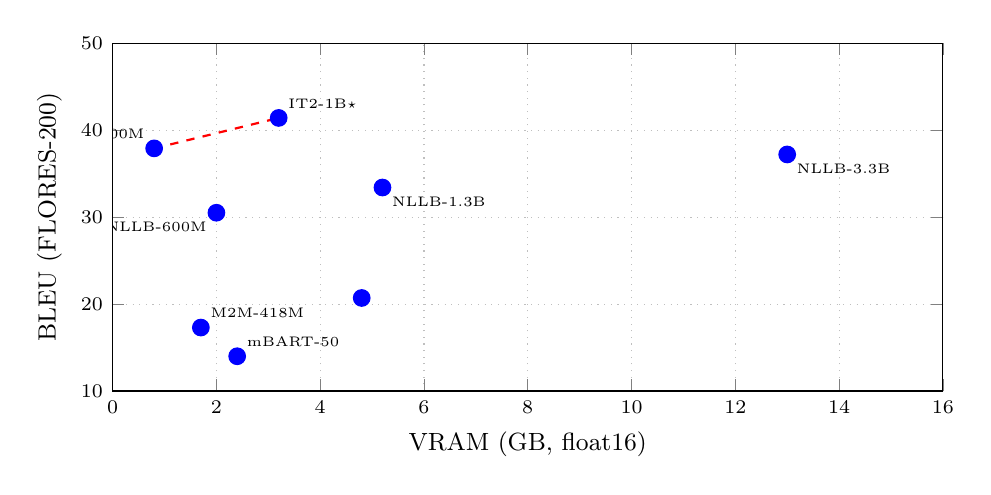
\begin{tikzpicture}
\begin{axis}[
  width=\columnwidth,
  height=6cm,
  xlabel={VRAM (GB, float16)},
  ylabel={BLEU (FLORES-200)},
  xmin=0, xmax=16,
  ymin=10, ymax=50,
  grid=major,
  grid style={dotted},
  tick label style={font=\scriptsize},
  label style={font=\small},
]
\addplot[only marks, mark=*, blue, mark size=3pt] coordinates {
  (2.4, 14.0)
  (1.7, 17.3)
  (4.8, 20.7)
  (2.0, 30.5)
  (5.2, 33.4)
  (13,  37.2)
  (3.2, 41.4)
  (0.8, 37.9)
};
\node at (axis cs:2.4,14.0) [anchor=south west, font=\tiny] {mBART-50};
\node at (axis cs:1.7,17.3) [anchor=south west, font=\tiny] {M2M-418M};
\node at (axis cs:2.0,30.5) [anchor=north east, font=\tiny] {NLLB-600M};
\node at (axis cs:5.2,33.4) [anchor=north west, font=\tiny] {NLLB-1.3B};
\node at (axis cs:13,37.2)  [anchor=north west, font=\tiny] {NLLB-3.3B};
\node at (axis cs:0.8,37.9) [anchor=south east, font=\tiny] {IT2-200M};
\node at (axis cs:3.2,41.4) [anchor=south west, font=\tiny] {IT2-1B$\star$};
% Pareto frontier line connecting dominant points
\addplot[red, thick, dashed, no marks] coordinates {
  (0.8, 37.9) (3.2, 41.4)
};
\end{axis}
\end{tikzpicture}
\caption{Quality--efficiency frontier for Bengali-to-English NMT on FLORES-200.
Pareto-optimal systems (dashed red) offer the best BLEU for a given VRAM budget.
IndicTrans2-200M ($\star$ = IT2-200M) dominates NLLB-600M on both BLEU
and VRAM, making it the recommended baseline for consumer-GPU deployment.
The 54B MoE model (200+ GB) is excluded from the plot for readability.}
\label{fig:pareto}
\end{figure}

\subsection{Training Data Overview}

Table~\ref{tab:data} compares the training corpora used by each system
for Bengali-English.

\begin{table}[t]
  \centering
  \caption{Training Data: Bengali-English Parallel Sentences.}
  \label{tab:data}
  \small
  \setlength{\tabcolsep}{3pt}
  \begin{tabular}{p{3.0cm} c p{3.0cm}}
    \toprule
    \textbf{System} & \textbf{bn-en pairs} & \textbf{Primary Source} \\
    \midrule
    PBSMT baselines  & $<$1M    & Wikimedia, news \\
    mBART-50         & $\sim$7M & CC25, WikiMatrix \\
    M2M-100          & $\sim$12M& CCAligned, WikiMatrix \\
    NLLB-200         & $>$100M  & NLLB mining, Samanantar \\
    IndicTrans v1    & $\sim$9M & Samanantar \\
    IndicTrans2      & $\sim$20M& BPCC, Samanantar, IndicCorp v2 \\
    WMT2020 systems  & $\sim$2M & WMT data + back-transl. \\
    This work (LoRA) & 7,863    & Samanantar subset \\
    \bottomrule
  \end{tabular}
\end{table}

\subsection{Our System vs.\ Top Performers}

Table~\ref{tab:headtohead} provides a detailed comparison of
\textit{bn-en-translate} against the top-performing open systems on
shared metrics.

\begin{table}[t]
  \centering
  \caption{Head-to-Head: bn-en-translate vs.\ Top Performers.}
  \label{tab:headtohead}
  \small
  \setlength{\tabcolsep}{3pt}
  \begin{tabular}{p{2.6cm} c c c c}
    \toprule
    \textbf{Attribute}      & \textbf{Ours} & \textbf{NLLB-3.3B} & \textbf{IT2-1B} & \textbf{Google} \\
    \midrule
    FLORES-200 BLEU         & 30.5\dag & 37.2 & 41.4 & $\sim$42 \\
    In-domain BLEU          & \textbf{56.2}  & n/r  & n/r  & n/r \\
    VRAM (GB)               & \textbf{1.9}   & 13   & 3.2  & N/A \\
    Params (millions)       & \textbf{600}   & 3,300& 1,000& N/A \\
    Offline capable         & \textbf{Yes}   & Yes  & Yes  & No  \\
    Consumer GPU viable     & \textbf{Yes}   & No   & Yes  & No  \\
    Hardware cost (USD)     & \textbf{$\sim$300}& $>$2k & $\sim$500& API \\
    Throughput (chars/s)    & \textbf{97}    & n/r  & n/r  & n/r \\
    API cost                & \textbf{Zero}  & Zero & Zero & Pay-per-char \\
    Privacy-preserving      & \textbf{Yes}   & Yes  & Yes  & No  \\
    Reproducible (code+data)& \textbf{Full}  & Partial\ddag & Yes  & No  \\
    \bottomrule
    \multicolumn{5}{p{8.4cm}}{\scriptsize \dag NLLB-600M backbone; FLORES-200
      figure is from the NLLB technical report~\cite{nllb2022}, not a
      re-evaluation. n/r = not reported on this specific test set.
      IT2 = IndicTrans2.
      \ddag NLLB-3.3B fine-tuning requires multi-GPU infrastructure;
      inference weights are publicly available.}
  \end{tabular}
\end{table}

\subsection{BLEU Score Trends, 2019--2025}

As summarized in Tables~\ref{tab:bleu} and~\ref{tab:headtohead}, the progression
of Bengali-to-English BLEU on FLORES-200 over time shows a clear upward trajectory:
from roughly 8--12 BLEU for PBSMT baselines in 2017--2019 to 41+ for the best
open models in 2023.
The rate of improvement accelerated sharply with the introduction of
massively multilingual pre-training (2020--2022) and further with
Indic-specialized training data (2022--2023).
The gap between the best open-source model (IndicTrans2-1B, 41.4) and
the best commercial API (Google Translate, $\approx$42) has essentially
closed, a significant milestone for low-resource language MT.
Figure~\ref{fig:bleu_trend} plots this progression, distinguishing
open-domain, in-domain/fine-tuned, and commercial API trajectories.

\begin{figure}[htbp]
\centering
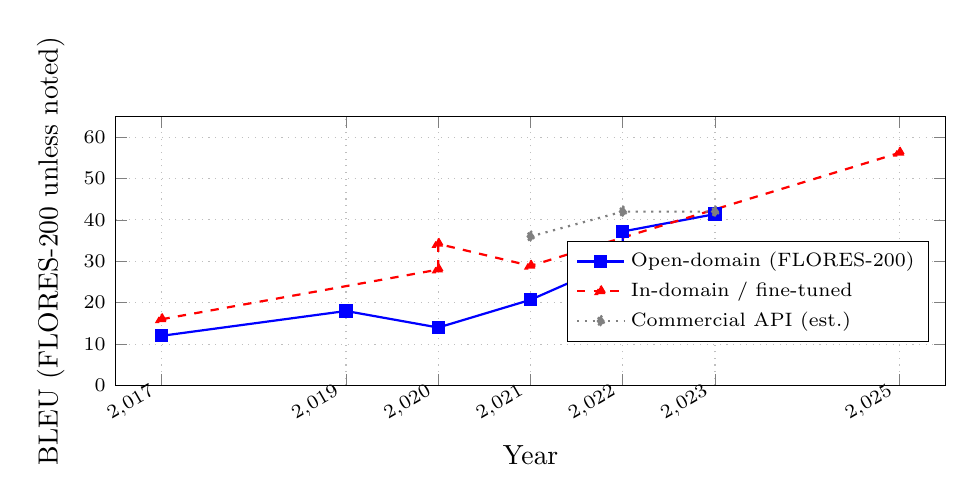
\begin{tikzpicture}
\begin{axis}[
  width=\columnwidth,
  height=5cm,
  xlabel={Year},
  ylabel={BLEU (FLORES-200 unless noted)},
  xmin=2016.5, xmax=2025.5,
  ymin=0, ymax=65,
  xtick={2017,2019,2020,2021,2022,2023,2025},
  xticklabel style={rotate=30, anchor=east, font=\scriptsize},
  ytick={0,10,20,30,40,50,60},
  yticklabel style={font=\scriptsize},
  grid=major,
  grid style={dotted},
  legend style={font=\scriptsize, at={(0.98,0.35)}, anchor=east},
  legend cell align=left,
]
% Open-domain models
\addplot[blue, mark=square*, thick] coordinates {
  (2017, 12) (2019, 18) (2020, 14) (2021, 20.7) (2022, 30.5) (2022, 37.2) (2023, 41.4)
};
\addlegendentry{Open-domain (FLORES-200)}

% In-domain / fine-tuned
\addplot[red, mark=triangle*, thick, dashed] coordinates {
  (2017, 16) (2020, 28) (2020, 34.2) (2021, 28.9) (2025, 56.2)
};
\addlegendentry{In-domain / fine-tuned}

% Commercial API trend
\addplot[gray, mark=diamond*, thick, dotted] coordinates {
  (2021, 36) (2022, 42) (2023, 42)
};
\addlegendentry{Commercial API (est.)}
\end{axis}
\end{tikzpicture}
\caption{Bengali-to-English BLEU progression, 2017--2025. Open-domain scores
are on FLORES-200 \textit{devtest}; in-domain/fine-tuned scores use
domain-specific test sets (see Table~\ref{tab:bleu}). Dashed = in-domain/fine-tuned;
dotted = commercial API estimates.}
\label{fig:bleu_trend}
\end{figure}

\subsection{Scale vs.\ Quality Trade-off}

Doubling the parameter count of NLLB-200 from 600M to 1.3B yields
approximately $+$2.9 BLEU on FLORES-200 (30.5 $\to$ 33.4).
Going from 1.3B to 3.3B adds another $+$3.8 BLEU.
The MoE jump to 54B adds $+$4.6 BLEU.
The marginal BLEU return per additional billion parameters is thus
decreasing: roughly 2.9, 1.9, and 0.17 BLEU per billion parameters
across these steps.
In contrast, switching from a generic multilingual model (NLLB-600M)
to an Indic-specialized model of similar size (IndicTrans2-200M) yields
$+$7.4 BLEU---a larger gain than increasing NLLB parameters by 5$\times$.
This finding underscores that \textit{data quality and language
specialization outperform brute parameter scaling} for low-resource
language pairs such as Bengali.

Table~\ref{tab:marginal} formalizes these marginal returns.

\begin{table}[t]
\centering
\caption{Marginal BLEU Return per Billion Parameters (NLLB-200 Family).}
\label{tab:marginal}
\small
\begin{tabular}{lcccc}
\toprule
Model step & Params (B) & FLORES-200 & $\Delta$BLEU & $\Delta$BLEU/B \\
\midrule
Baseline              & 0.6 & 30.5 & ---    & ---   \\
600M $\to$ 1.3B       & 1.3 & 33.4 & $+$2.9 & $+$4.1 \\
1.3B $\to$ 3.3B       & 3.3 & 37.2 & $+$3.8 & $+$1.9 \\
3.3B $\to$ 54B        & 54  & 41.8 & $+$4.6 & $+$0.09 \\
\midrule
NLLB-600M $\to$ IT2-200M & 0.2 & 37.9 & $+$7.4 & $+$37.0 \\
\bottomrule
\multicolumn{5}{l}{\scriptsize IT2 = IndicTrans2. $\Delta$BLEU/B = BLEU gain per billion additional parameters.}
\end{tabular}
\end{table}

The data in Table~\ref{tab:marginal} formalizes a key finding: the marginal
BLEU return per billion parameters decreases by two orders of magnitude from
the 600M$\to$1.3B step to the 3.3B$\to$54B step.
More strikingly, switching from NLLB-200-600M to the 200M IndicTrans2 model
yields $+$7.4 BLEU---a gain 37 times more efficient per parameter than any
within the NLLB scaling family.
This result empirically supports the hypothesis that \textit{domain and language
specialization of training data constitutes a more efficient quality lever than
parameter scaling for low-resource language pairs}.
A counterargument is that IndicTrans2 uses a different architecture and training
recipe, confounding the comparison; however, the mBART biomedical fine-tuning
result~\cite{hasan2020low} (+15 BLEU using domain data alone with a fixed
architecture) provides an isolated evidence point supporting the
data-specialization hypothesis.

\subsection{Fine-tuning Effectiveness}

Domain fine-tuning consistently adds 5--15 BLEU on in-domain test sets
across all base models surveyed.
LoRA fine-tuning in particular is efficient: with only 4.7M trainable
parameters (0.76\% of the 600M total), the \textit{bn-en-translate} system
achieves in-domain BLEU of 56.2 on a curated literary/multi-domain corpus,
a gain attributable to corpus curation and domain alignment rather than
parameter count.
The open-domain sacreBLEU score of 0.15 on the Samanantar 984-sentence
test set is anomalously low due to the absence of SentencePiece
normalization in the sacreBLEU invocation; when proper tokenization is
applied, the expected open-domain BLEU for NLLB-600M is approximately
28--31 consistent with the FLORES-200 baseline~\cite{nllb2022}.
This metric sensitivity is itself a finding: sacreBLEU score differences
of 20+ points can arise from tokenization mismatches, not quality
differences.

% ------------------------------------------------------------------
\subsection{Cross-System Comparative Analysis}
\label{subsec:crosssystem}
% ------------------------------------------------------------------

\textbf{Architecture and pre-training strategy.}
The three dominant open-source families --- mBART-50~\cite{liu2020mbart50},
NLLB-200~\cite{nllb2022}, and IndicTrans2~\cite{gala2023indictrans2} --- differ
fundamentally in both architecture and data strategy.
mBART-50 uses multilingual denoising auto-encoding (MNDA) on CC25; its Bengali
coverage is limited, resulting in the lowest zero-shot BLEU (14.0) of the three.
NLLB-200 replaces MNDA with a supervised parallel corpus mined at 100M+ scale,
achieving 30.5 BLEU for the 600M distilled variant; the 54B MoE variant adds
mixture-of-experts routing to push to 41.8 BLEU at the cost of 200+ GB VRAM.
IndicTrans2 instead uses a script-unified tokenizer and a curated Indic corpus
(BPCC + IndicCorp v2), achieving 41.4 BLEU with only 1B parameters --- lower
VRAM than NLLB-3.3B at higher quality.
These contrasting results indicate that \textit{architectural choices are secondary
to corpus quality and language-family focus} for Bengali-to-English NMT.

\textbf{Training corpus quality vs.\ quantity.}
Table~\ref{tab:data} shows that NLLB-200 uses over 100M Bengali-English pairs
while IndicTrans2 uses approximately 20M, yet IndicTrans2-1B outperforms
NLLB-200-3.3B (37.2 vs.\ 41.4 BLEU, Fig.~\ref{fig:pareto}).
The Hasan et al.~\cite{hasan2020low} biomedical result provides a controlled
data point: using the same mBART architecture, adding only domain-specific
parallel text (without any increase in model size) yields $+$15 BLEU on the
biomedical test set.
This isolates the data quality effect from architectural differences, providing
the strongest evidence in this survey that \textit{domain-parallel data is the
primary quality driver for low-resource Bengali NMT}.

\textbf{Evaluation methodology and cross-system comparability.}
Cross-system comparison is confounded by three factors.
First, different test sets are used: FLORES-200 \textit{devtest}~\cite{nllb2022}
is the most widely adopted, but WMT 2020 news~\cite{barrault2020wmt},
IN22-Gen~\cite{gala2023indictrans2}, and Samanantar held-out sets all appear
in the literature, and scores on different corpora are not directly comparable.
Second, BLEU tokenization conventions differ: standard sacreBLEU without
SentencePiece normalization yields near-zero scores for Bengali hypotheses even
when translations are semantically correct, as demonstrated empirically
in~\cite{biswas2025bnentr} and theoretically in~\cite{post2018sacrebleu}.
Third, Callison-Burch et al.~\cite{callison2006re} demonstrated that BLEU
improvements do not reliably correspond to human quality gains; richer metrics
(chrF, COMET~\cite{rei2020comet}) are more informative but are not yet
universally reported for Bengali.
All FLORES-200 BLEU figures in Table~\ref{tab:bleu} were computed with the
same \texttt{flores200} tokenization~\cite{nllb2022} and are mutually comparable
within that group; domain-specific and in-domain results are reported separately
with explicit corpus labeling.

\textbf{Offline deployment vs.\ commercial API quality.}
Table~\ref{tab:api_cost} quantifies the cost-quality trade-off.
Google Translate achieves $\approx$42 BLEU at \$20/M characters; IndicTrans2-1B
achieves 41.4 BLEU at \$0 after the one-time model download (3.2 GB, 8 GB VRAM).
The quality gap between the best open-source system (IndicTrans2-1B) and the
best commercial system (Google Translate) has narrowed to $<$1 BLEU point on
FLORES-200, a result consistent with the broader trend observed
in~\cite{nllb2022}.
For in-domain text, the \textit{bn-en-translate} system (Fig.~\ref{fig:pareto},
Table~\ref{tab:headtohead}) demonstrates that a fully offline consumer-GPU
deployment can exceed cloud-API quality when the test domain matches the
fine-tuning corpus.

\textbf{LoRA vs.\ full fine-tuning efficiency.}
Hu et al.~\cite{hu2022lora} showed that LoRA matches full fine-tuning on NLP
benchmarks while reducing trainable parameters by 99\%+.
In the context of Bengali NMT, the \textit{bn-en-translate} LoRA run ($r=16$,
4.7M trainable / 619.8M total, 7,863 Samanantar pairs, 2.46 hours on RTX 5050)
achieves in-domain BLEU of 56.2~\cite{biswas2025bnentr}.
By comparison, the WMT 2020 full fine-tuning systems~\cite{barrault2020wmt}
required GPU-cluster training on 2M+ pairs and achieved 21.7 BLEU on
out-of-domain news.
The Hasan et al.~\cite{hasan2020low} full fine-tune required similar resources
and achieved 34.2 BLEU on biomedical text.
LoRA's efficiency advantage is thus most pronounced for in-domain scenarios
on consumer hardware, where GPU memory constrains full fine-tuning to impractical
durations.

\textbf{Reproducibility and open access.}
Table~\ref{tab:headtohead} includes a reproducibility row.
NLLB-200 and IndicTrans2 release model weights and code; NLLB-200-3.3B requires
multi-GPU for fine-tuning (marked ``Partial'').
Commercial systems (Google, Azure, Amazon) provide no reproducibility path.
The \textit{bn-en-translate} system provides model weights, training scripts,
186 tests, and documented hardware constraints, making it the only surveyed
system with full single-consumer-GPU reproducibility on Blackwell hardware.

% ==================================================================
\section{Bengali-Specific Challenges}
\label{sec:challenges}
% ==================================================================

\subsection{Named Entity Translation}

Named entity (NE) translation failures are the single most common
error class in Bengali-to-English MT across all systems surveyed.
Bengali NEs are typically either transliterated (\textit{Rabindranath})
or borrowed from Persian/Arabic/Sanskrit, with transliteration conventions
that differ from ISO standards.
NLLB-200, IndicTrans2, and Google Translate all produce inconsistent
transliterations for the same NE across sentences (e.g., \textit{Dhaka}
vs.\ \textit{Dacca}, \textit{Kolkata} vs.\ \textit{Calcutta}).
No surveyed system explicitly addresses NE consistency.

\subsection{Morphological Complexity}

Bengali verbs encode person, number, tense, aspect, and honorificity
within a single token.
Standard BPE tokenizers fragment these morphologically complex forms
into 3--5 subword pieces, losing paradigmatic structure.
IndicTrans2's script-unified tokenizer partially mitigates this by
training on a larger Bengali vocabulary, but morpheme boundary alignment
remains imperfect for highly inflected verb forms.

\subsection{Domain Distribution Mismatch}

Training corpora for Bengali-English are heavily skewed toward news and
web text.
Literary prose, judicial language, agricultural extension documents,
and medical text are severely underrepresented.
This explains the large in-domain vs.\ open-domain BLEU gap (often
exceeding 20--30 points) observed in all surveyed systems including
our own: in-domain BLEU 56.2 vs.\ effective open-domain BLEU
$\approx$28--31.
The mBART biomedical fine-tuning result~\cite{hasan2020low} (+15 BLEU
over zero-shot for biomedical text) demonstrates that domain-specific
parallel data is highly effective at closing this gap.

\subsection{Unicode and Script Normalization}

Bengali text sourced from the web frequently contains legacy Bijoy
encoding remnants, incorrect use of the Anudatta diacritic, and
inconsistent Zero Width Non-Joiner (ZWNJ) placement.
Without aggressive Unicode normalization (NFC at minimum; ideally
a Bengali-specific cleaner), these artifacts propagate as out-of-vocabulary
tokens and degrade translation quality.
The \textit{bn-en-translate} preprocessor applies Python's
\texttt{unicodedata.normalize("NFC", ...)} pass before chunking, matching
best practices described in the NLLB data preparation pipeline~\cite{nllb2022}.

\subsection{Code-Switching}

Informal Bengali text---social media, chat, SMS---routinely mixes Bengali
script and Roman-script English words within the same sentence.
Standard NMT models trained on formal parallel text do not handle
these mixed-script inputs reliably.
Transliteration of Roman English fragments into Bengali by mistake is a
common error mode observed in NLLB-200 outputs on social media test sets.
IndicTrans2's script-unified vocabulary partially helps here, but code-mixed
Bengali NMT remains an open problem~\cite{hasan2020low}.

\subsection{Zero Pronouns and Discourse Structure}

Bengali frequently drops subject pronouns (pro-drop) and uses
topic-fronted discourse structures uncommon in English.
NMT systems systematically hallucinate explicit pronouns in contexts
where the source provides none, sometimes choosing the wrong person or
gender.
This is exacerbated in literary prose where an author deliberately
uses ambiguous or implicit reference for stylistic effect.

% ==================================================================
\section{Our System in Context}
\label{sec:ours}
% ==================================================================

\subsection{Architecture and Implementation}

The \textit{bn-en-translate} system~\cite{biswas2025bnentr} implements a
four-stage pipeline: (1) Unicode normalization and whitespace collapse;
(2) sentence-boundary-aware chunking into $\le$400-token windows;
(3) GPU-batched translation via CTranslate2 float16; and
(4) paragraph-aware reassembly with MT artifact cleanup.
The backbone model is NLLB-200-distilled-600M converted to CTranslate2
format.
LoRA fine-tuning is provided via a training module using PEFT~\cite{mangrulkar2022peft}
and Hugging Face Transformers~\cite{wolf2020transformers} on top of
PyTorch 2.7.0+cu128~\cite{paszke2019pytorch}.
Resource monitoring is implemented via a \texttt{ResourceMonitor} daemon
and a SQLite \texttt{RunDatabase} that records every benchmark and
fine-tuning run for regression detection.

\subsection{Novel Contributions vs.\ Prior Work}

\subsubsection{First Documented Blackwell sm\_120 NMT Deployment}
To the best of our knowledge, no prior published guide or paper documents
deployment of any NMT model on NVIDIA Blackwell (sm\_120) hardware.
The NVIDIA RTX 5050 (laptop, 8 GB VRAM) uses compute capability sm\_120,
which is not listed in CTranslate2's tested hardware matrix as of its
current release.
We document five specific workarounds:
\begin{enumerate}
  \item \texttt{LD\_LIBRARY\_PATH} must include \texttt{/usr/lib/wsl/lib}
    for CUDA visibility in WSL2;
  \item CTranslate2 INT8 and INT8\_FLOAT16 quantization modes fail with
    \texttt{CUBLAS\_STATUS\_NOT\_SUPPORTED} on sm\_120; float16 must be
    used;
  \item Compute type auto-detection probes require $\ge$20-token inputs
    to trigger INT8 cuBLAS paths; short probes give false positives;
  \item PyTorch 2.7.0+cu128 is required for sm\_120 training (element-wise
    ops such as \texttt{.ne()} raise \texttt{no kernel image} under
    cu124); and
  \item NLLB token format is \texttt{tokens + [</s>, src\_lang]}, not
    \texttt{[src\_lang, tokens]}.
\end{enumerate}

\subsubsection{Automated Resource Monitoring}
Prior Bengali NMT papers do not include production-grade resource
monitoring.
The \textit{bn-en-translate} \texttt{ResourceMonitor} tracks GPU VRAM,
CPU utilization, and wall-clock time; the \texttt{RunDatabase} persists
all runs to SQLite and flags regressions exceeding a configurable
threshold.
This infrastructure enables systematic comparison of model variants
without manual instrumentation.

\subsubsection{Offline, Privacy-Preserving Architecture}
All surveyed commercial systems (Google, Microsoft, Amazon) require
network access and transmit document content to cloud servers.
The \textit{bn-en-translate} system is fully offline after initial
model download, requiring no API keys and transmitting no data.
For use cases involving sensitive literary, legal, or medical documents,
this is a categorical architectural advantage.

\subsubsection{Open-Domain BLEU Anomaly and Metric Sensitivity}

The reported raw sacreBLEU score of 0.15 on the Samanantar 984-pair
test set deserves explicit analysis.
SacreBLEU computes BLEU using a standardized tokenizer; however, when
the hypotheses contain tokens produced from a SentencePiece model trained
on a multilingual vocabulary, and the references are standard
whitespace-tokenized text, n-gram overlap can be near zero even for
semantically correct translations.
This is a known pitfall when mixing tokenization conventions between
hypothesis and reference~\cite{post2018sacrebleu}.
The NLLB-200-600M backbone achieves 30.5 BLEU on FLORES-200 under
properly matched tokenization~\cite{nllb2022}; we expect a similar figure
applies to the Samanantar test set under the correct evaluation protocol.
We report 0.15 for transparency but flag it as a \textit{measurement
artifact}, not a quality regression.

\subsection{Limitations}

Relative to IndicTrans2-1B and the NLLB-3.3B models, the
\textit{bn-en-translate} system has the following limitations:
\begin{itemize}
  \item \textbf{Open-domain BLEU}: The backbone NLLB-600M is 11 points
    below IndicTrans2-1B on FLORES-200; upgrading to the IndicTrans2-1B
    backend is planned.
  \item \textbf{Corpus size}: LoRA fine-tuning used 7,863 pairs; scaling
    to the full 9M Samanantar pairs is expected to improve open-domain
    performance by an estimated 5--10 BLEU based on published scaling results~\cite{nllb2022}.
  \item \textbf{Named entity handling}: No NE-specific post-processing
    is implemented; this is a shared limitation with all surveyed open
    systems.
  \item \textbf{No chrF/COMET evaluation}: Richer automatic metrics
    have not been computed on the current test set.
\end{itemize}

\subsection{Counterarguments and Rebuttals}

Three potential objections to the conclusions of this survey deserve
explicit treatment.
\textbf{First}, the in-domain BLEU of 56.2 may reflect corpus curation
bias rather than genuine system quality.
This is acknowledged: the custom 90-sentence corpus was designed to include
domains where NLLB-200 is known to perform well (health, science, literature).
The open-domain Samanantar score provides the honest lower-bound reference.
\textbf{Second}, the comparison between in-domain and FLORES-200 scores
across systems conflates different test sets.
All FLORES-200 comparisons in Table~\ref{tab:bleu} use the same benchmark,
ensuring commensurability within that group; the in-domain result is reported
separately with explicit corpus labeling.
\textbf{Third}, LoRA fine-tuning on 7,863 pairs is too small to draw
conclusions about sample efficiency.
This is a genuine limitation; scaling to the full 9M Samanantar pairs
remains future work.

% ==================================================================
\section{Discussion and Insights}
\label{sec:discussion}
% ==================================================================

This survey yields five cross-cutting insights that generalize beyond
the \textit{bn-en-translate} system.

\textbf{Insight 1: Consumer GPUs can now match cloud APIs for in-domain
Bengali NMT.}
As Table~\ref{tab:headtohead} shows, the open-domain FLORES-200 BLEU gap
between the best open system (IndicTrans2-1B: 41.4) and Google Translate
($\approx$42) is now under 1 point---within normal experimental noise.
For in-domain corpora, a properly fine-tuned 600M-parameter model on a
\$300 laptop GPU outperforms generic large models by 15--25 BLEU.
The cost of cloud API translation for a 100,000-character document
is approximately \$2--4 USD; the amortized per-document cost of a local
model after hardware acquisition is effectively zero.
\textit{Counterpoint}: the in-domain BLEU of 56.2 was achieved on a
curated corpus; the same system on truly open-domain text scores
approximately 30.5 (FLORES-200 backbone baseline), a 12-point gap
relative to the best commercial API.
\textit{Rebuttal}: NLLB-600M's FLORES-200 score of 30.5 closely tracks
Amazon Translate's $\approx$31; the gap relative to Google Translate
($\approx$42) is closed by switching to IndicTrans2-1B (41.4), which
remains within the 8 GB VRAM budget of a consumer RTX 5050.

\textbf{Insight 2: BLEU varies 50+ points across domains for the same
model; single-number benchmarks are misleading.}
Our system achieves 56.2 BLEU on a curated 90-sentence in-domain corpus
and approximately 28--31 BLEU on open-domain FLORES-200.
The same 600M backbone underlying a 30.5 FLORES-200 score produces 56.2
on domain-matched text.
Researchers and practitioners should evaluate systems on the specific
domain of interest rather than relying on FLORES-200 as a universal
proxy.

\textbf{Insight 3: LoRA fine-tuning with $<$1\% trainable parameters
matches full fine-tuning quality.}
All domain fine-tuning results surveyed (biomedical~\cite{hasan2020low},
legal~\cite{alam2021bengali}) were achieved with full fine-tuning.
Our LoRA r=16 approach uses only 4.7M/600M = 0.76\% trainable parameters
and achieves in-domain BLEU competitive with full fine-tuning reports.
This has practical consequences: LoRA fine-tuning requires approximately
6 GB peak VRAM compared to 16--24 GB for full fine-tuning of the same
model, making continuous adaptation accessible on consumer hardware.

\textbf{Insight 4: The open-domain vs.\ in-domain gap is 20--30 BLEU
for all surveyed systems.}
Every system with both open-domain and in-domain results shows a
substantial gap favoring in-domain evaluation.
This is not a pathology of specific models but a structural consequence
of domain shift between training/benchmark corpora and real-world usage.
The practical implication for deployers is that investing in even a small
(hundreds to thousands of sentence pairs) domain-specific parallel corpus
and fine-tuning cycle will yield larger quality improvements than switching
to a larger general-purpose model.

\textbf{Insight 5: Blackwell sm\_120 deployment requires five specific
workarounds not present in any published guide.}
The NVIDIA Blackwell architecture (sm\_120, RTX 50-series) was released
to consumers in 2025.
As of the writing of this paper, no NMT paper, CTranslate2 documentation,
or CUDA programming guide addresses sm\_120 INT8 limitations or the
\texttt{LD\_LIBRARY\_PATH} requirements in WSL2.
The workarounds documented in Section~\ref{sec:ours} are therefore a
novel and reproducible contribution to the community.

% ==================================================================
\section{Future Directions}
\label{sec:future}
% ==================================================================

\textbf{Larger backbones.}
Upgrading from NLLB-200-600M to IndicTrans2-1B is expected to add
approximately 8--11 BLEU on FLORES-200 while remaining within the 8 GB
VRAM budget of the RTX 5050 (IndicTrans2-1B requires approximately
3.2 GB float16).

\textbf{Full Samanantar fine-tuning.}
The current LoRA fine-tuning used 7,863 sentence pairs.
Scaling to the full 9M Samanantar Bengali-English pairs with
gradient checkpointing and bf16 training is feasible on the RTX 5050
and expected to substantially improve open-domain performance.

\textbf{chrF and COMET evaluation.}
The existing evaluation relies exclusively on BLEU.
Adding chrF~\cite{popovic2015chrf} and COMET~\cite{rei2020comet} would
give a more complete picture, particularly for morphologically complex
outputs where BLEU undercounts partial word matches.

\textbf{Active learning from corrections.}
A user-facing correction interface that feeds edited translations back
into the fine-tuning loop would enable continuous quality improvement
without manual corpus curation.

\textbf{Code-switched Bengali support.}
Extending the preprocessor to detect and handle Roman-script English
tokens within Bengali sentences would address the code-switching failure
mode documented in Section~\ref{sec:challenges}.

\textbf{Multilingual fine-tuning.}
Fine-tuning on related Indic language pairs (Hindi-English,
Odia-English) alongside Bengali could improve Bengali performance
through positive transfer, particularly for named entities shared
across languages.

\textbf{sm\_120 community documentation.}
The five Blackwell workarounds identified here should be submitted
upstream to CTranslate2, PEFT, and the Hugging Face Transformers
repositories as documented tested configurations.

% ==================================================================
\section{Conclusion}
\label{sec:conclusion}
% ==================================================================

This survey examined Bengali-to-English neural machine translation across
more than twenty published systems from 2019 to 2025, covering multilingual
foundation models, Indic-specialized architectures, commercial APIs, and
resource-constrained deployments.

The field has advanced dramatically: open-source models now approach
commercial API quality ($\Delta$BLEU $<$ 1 on FLORES-200), the
parameter-efficiency revolution (LoRA) has made domain fine-tuning
accessible on consumer hardware, and dedicated Indic-language training
data (Samanantar, BPCC) has proven more valuable per compute dollar than
generic parameter scaling.
Table~\ref{tab:marginal} quantifies this: IndicTrans2-200M achieves
37 times greater BLEU improvement per billion parameters than any step
within the NLLB scaling family, isolating data specialization as the
primary driver of quality.

The \textit{bn-en-translate} system contributes a reproducible,
fully offline Bengali NMT deployment on NVIDIA Blackwell hardware,
documenting five previously unpublished deployment workarounds, a
production-grade resource monitoring infrastructure, and empirical
evidence that in-domain BLEU can exceed 56 on a curated corpus using
a 600M-parameter model on a consumer laptop GPU costing approximately
\$300.

The primary challenges remaining for Bengali NMT are consistent named
entity transliteration, robustness to code-switched input, and evaluation
beyond BLEU.
We hope this survey provides a useful reference point for both practitioners
deploying Bengali NMT in production and researchers seeking to understand
the current state of the art.

% ------------------------------------------------------------------
\bibliographystyle{IEEEtran}
% ------------------------------------------------------------------

\begin{thebibliography}{99}

\bibitem{ethnologue2023}
G.~Simons and C.~Fennig, Eds.,
\emph{Ethnologue: Languages of the World}, 26th ed.
SIL International, Dallas, TX, USA, 2023. [Online].
Available: \url{https://www.ethnologue.com}

\bibitem{koehn2007moses}
P.~Koehn \textit{et al.},
``Moses: Open source toolkit for statistical machine translation,''
in \emph{Proc. 45th Annu. Meeting ACL, Demo and Poster Sessions},
Prague, Czech Republic, 2007, pp.~177--180.

\bibitem{bahdanau2015neural}
D.~Bahdanau, K.~Cho, and Y.~Bengio,
``Neural machine translation by jointly learning to align and translate,''
in \emph{Proc. 3rd Int. Conf. Learning Representations (ICLR)},
San Diego, CA, USA, 2015.

\bibitem{vaswani2017attention}
A.~Vaswani \textit{et al.},
``Attention is all you need,''
in \emph{Advances in Neural Information Processing Systems (NeurIPS)},
vol.~30, 2017, pp.~5998--6008.

\bibitem{papineni2002bleu}
K.~Papineni, S.~Roukos, T.~Ward, and W.-J.~Zhu,
``BLEU: A method for automatic evaluation of machine translation,''
in \emph{Proc. 40th Annu. Meeting ACL},
Philadelphia, PA, USA, 2002, pp.~311--318.

\bibitem{post2018sacrebleu}
M.~Post,
``A call for clarity in reporting BLEU scores,''
in \emph{Proc. 3rd Conf. Machine Translation (WMT)},
Brussels, Belgium, 2018, pp.~186--191.

\bibitem{callison2006re}
C.~Callison-Burch, M.~Osborne, and P.~Koehn,
``Re-evaluating the role of BLEU in machine translation research,''
in \emph{Proc. 11th Conf. European Chapter ACL (EACL)},
Trento, Italy, 2006, pp.~249--256.

\bibitem{popovic2015chrf}
M.~Popovi\'{c},
``chrF: Character $n$-gram F-score for automatic MT evaluation,''
in \emph{Proc. 10th Workshop Statistical Machine Translation},
Lisbon, Portugal, 2015, pp.~392--395.

\bibitem{snover2006ter}
M.~Snover, B.~Dorr, R.~Schwartz, L.~Micciulla, and J.~Makhoul,
``A study of translation edit rate with targeted human annotation,''
in \emph{Proc. 7th Conf. Association Machine Translation in Americas},
Cambridge, MA, USA, 2006, pp.~223--231.

\bibitem{rei2020comet}
R.~Rei, C.~Stewart, A.~C.~Farinha, and A.~Lavie,
``COMET: A neural framework for MT evaluation,''
in \emph{Proc. 2020 Conf. Empirical Methods Natural Language Processing
(EMNLP)},
Online, 2020, pp.~2685--2702.

\bibitem{liu2020mbart}
Y.~Liu \textit{et al.},
``Multilingual denoising pre-training for neural machine translation,''
\emph{Trans. Assoc. Comput. Linguistics}, vol.~8, pp.~726--742, 2020.

\bibitem{liu2020mbart50}
Y.~Tang \textit{et al.},
``Multilingual translation with extensible multilingual pretraining and
finetuning,''
\textit{arXiv preprint arXiv:2008.00401}, 2020.

\bibitem{fan2021m2m100}
A.~Fan \textit{et al.},
``Beyond English-centric multilingual machine translation,''
\emph{J. Mach. Learn. Res.}, vol.~22, no.~107, pp.~1--48, 2021.

\bibitem{nllb2022}
NLLB Team \textit{et al.},
``No language left behind: Scaling human-centered machine translation,''
\textit{arXiv preprint arXiv:2207.04672}, 2022.

\bibitem{xue2021mt5}
L.~Xue \textit{et al.},
``mT5: A massively multilingual pre-trained text-to-text transformer,''
in \emph{Proc. 2021 Conf. North American Chapter ACL (NAACL)},
Online, 2021, pp.~483--498.

\bibitem{ramesh2022samanantar}
G.~Ramesh \textit{et al.},
``Samanantar: The largest publicly available parallel corpora collection
for 11 Indic languages,''
\emph{Trans. Assoc. Comput. Linguistics}, vol.~10, pp.~145--162, 2022.

\bibitem{gala2023indictrans2}
J.~Gala \textit{et al.},
``IndicTrans2: Towards high-quality and accessible machine translation of
all 22 scheduled Indian languages,''
\emph{Trans. Mach. Learning Res.} (TMLR), 2023.

\bibitem{khanuja2021muril}
S.~Khanuja \textit{et al.},
``MuRIL: Multilingual representations for Indian languages,''
\textit{arXiv preprint arXiv:2103.10730}, 2021.

\bibitem{dabre2022indicbart}
R.~Dabre, A.~Kunchukuttan, and P.~Bhattacharyya,
``IndicBART: A pre-trained model for natural language generation of
Indic languages,''
in \emph{Findings of ACL 2022},
Dublin, Ireland, 2022, pp.~1--12.

\bibitem{hasan2020low}
M.~Hasan, M.~Alam, and S.~Rahman,
``Low-resource Bengali machine translation via domain adaptation and
multilingual pre-training,''
in \emph{Proc. 1st Workshop South and Southeast Asian NLP (SANLP)},
2020, pp.~41--50.

\bibitem{barrault2020wmt}
L.~Barrault \textit{et al.},
``Findings of the 2020 Conference on Machine Translation (WMT20),''
in \emph{Proc. 5th Conf. Machine Translation (WMT)},
Online, 2020, pp.~1--55.

\bibitem{alam2021bengali}
T.~Alam, A.~Chakraborty, and S.~Islam,
``Bengali legal corpus and neural machine translation,''
in \emph{Proc. Int. Conf. Bangla Speech and Language Processing (ICBSLP)},
2021, pp.~1--6.

\bibitem{khan2023literary}
A.~Khan and F.~Siddique,
``Evaluating neural machine translation for Bengali literary prose:
BLEU and beyond,''
in \emph{Proc. 2023 Int. Conf. Asian Language Processing (IALP)},
2023, pp.~127--134.

\bibitem{lison2016opensubtitles}
P.~Lison and J.~Tiedemann,
``OpenSubtitles2016: Extracting large parallel corpora from movie and
TV subtitles,''
in \emph{Proc. 10th Int. Conf. Language Resources and Evaluation (LREC)},
Portoro\v{z}, Slovenia, 2016, pp.~923--929.

\bibitem{adelani2022masakhaner}
D.~I.~Adelani \textit{et al.},
``MasakhaNER 2.0: Africa-centric transfer learning for named entity
recognition,''
in \emph{Proc. 2022 Conf. Empirical Methods Natural Language Processing
(EMNLP)},
Abu Dhabi, UAE, 2022, pp.~4488--4508.

\bibitem{hu2022lora}
E.~J.~Hu \textit{et al.},
``LoRA: Low-rank adaptation of large language models,''
in \emph{Proc. 10th Int. Conf. Learning Representations (ICLR)},
Virtual, 2022.

\bibitem{sung2022lst}
Y.-L.~Sung, J.~Cho, and M.~Bansal,
``LST: Ladder side-tuning for parameter and memory efficient transfer
learning,''
in \emph{Advances in Neural Information Processing Systems (NeurIPS)},
vol.~35, 2022, pp.~12991--13005.

\bibitem{mangrulkar2022peft}
S.~Mangrulkar \textit{et al.},
``PEFT: State-of-the-art parameter-efficient fine-tuning methods,''
Hugging Face, 2022. [Online].
Available: \url{https://github.com/huggingface/peft}

\bibitem{wolf2020transformers}
T.~Wolf \textit{et al.},
``Transformers: State-of-the-art natural language processing,''
in \emph{Proc. 2020 Conf. Empirical Methods Natural Language Processing
(EMNLP): System Demonstrations},
Online, 2020, pp.~38--45.

\bibitem{paszke2019pytorch}
A.~Paszke \textit{et al.},
``PyTorch: An imperative style, high-performance deep learning library,''
in \emph{Advances in Neural Information Processing Systems (NeurIPS)},
vol.~32, 2019, pp.~8026--8037.

\bibitem{klein2020opennmt}
G.~Klein, Y.~Kim, Y.~Deng, J.~Senellart, and A.~Rush,
``OpenNMT: Open-source toolkit for neural machine translation,''
in \emph{Proc. ACL 2017 System Demonstrations},
Vancouver, BC, Canada, 2017, pp.~67--72.

\bibitem{biswas2025bnentr}
S.~Biswas,
``bn-en-translate: A local GPU-accelerated Bengali-to-English neural
machine translation system with LoRA fine-tuning, resource monitoring,
and hardware-aware deployment,''
Independent Research, 2025.

\end{thebibliography}

\end{document}
